\subsubsection{Definition}
\label{sub:definition}

\begin{quote}
For thousands of years, we have tried to understand how we think; that is, how a mere handful of matter can perceive, understand, predict, and manipulate a world far larger and more complicated than itself. The field of artificial intelligence, or AI, goes further still: it attempts not just to understand but also to build intelligent entities.
\end{quote}

This is the quote used by Stuart Russel and Peter Norvig~\footcite{russell2016artificial} to introduce the field of \gls{ai} in their book “Artificial Intelligence: A modern approach“.

In order to give a clear overview of the topics of \gls{ml} and especially deep learning it is important to clearly separate terms that are commonly used interchangeably. While many different definitions for \gls{ai} can be found, it generally refers to the broader concept of creating general-purpose machines that can perform tasks that are characteristic of human intelligence. To achieve this, machines need to detect patterns in data they are fed and to build up knowledge from these patterns.

The fundamental goal of \gls{ml} is to develop a \textit{machine} or an \textit{algorithm} that \textit{learns} to perform a \textit{task} from \textit{past experience}. More abstractly, our goal is to learn a mapping from input to output
\begin{equation}
	f : I \rightarrow O
\end{equation}
which can also be written as
\begin{equation}
	y = f(x ; \theta)
\end{equation}
where $ x \in I $ denotes the input, $ y \in O $ denotes the output and $ \theta \in \Theta $ denotes the parameters of the model.

To have a well-functioning model, different steps have to be completed. First of all, we need proper inputs (and outputs) in the form of data entries suited for the problem. These data entries are then typically split into two subsets called the \textit{training} data and the \textit{test} data. Then, the training data is used to tune the model parameters, or \textit{weights}, to minimize the difference between the model prediction and the desired output. With the test data, one can evaluate how good the model is at performing the given task by comparing the prediction with the “true“ or the desired result. Hereby, \gls{ml} models are divided into different categories depending on either their type of problem and the format of their training (and test) data.

\paragraph*{Problem type}
The first distinction can be made along the value range of the output variable. If the model learns a mapping into a discrete space (e.g. \{1, 2, ..., 10\}), then we are talking about a \textbf{classification} problem. The perhaps most famous example for this task is the MNIST handwritten digit classification~\footnote{\url{http://yann.lecun.com/exdb/mnist/}}, where a model learns to recognize handwritten digits provided in the form of images. Another example could be the recognition of music genres given the audio input files. If, however, the model learns a mapping into a continuous space (e.g. $ O = {\rm I\!R} $) , then we are talking about a \textbf{regression} problem. For this problem, the prediction of the value of a house given certain features such as the property square meters or the location in the city (e.g. “good“ or “bad“) can be listed. \textbf{Density estimation} is the task of being confronted with data points for which one does not know the underlying distribution. Taking a look at the locations of a dart disk that a dart that was thrown several times landed on might show us that we are dealing with an inverse two-dimensional Gaussian distribution. The last problem type that will be listed is the one of \textbf{clustering}: Here, one is faced with data points and shall determine (the amount of) class types that best encapsulate groups within the data points. One such example could be a streaming provider that wants to determine what kinds of viewer groups it has to perform further marketing and personalization strategies. Other \gls{ml} task definitions and examples can be found in subject-specific literature or the internet.

\paragraph*{Data format}
In a \textbf{supervised learning} environment, both the input and the output data points are made available to the model. This allows us to compute a distance function between output and desired result, also called cost function (ch. 3.3.3). Using this cost function as a performance measure, the model is able to give more accurate predictions over time by optimizing the cost function at each step (see above classification and regression examples). In an \textbf{unsupervised learning} environment, we only get the raw data entries without the desired output, or \textit{labels}. As we, therefore, have no metric for calculating the distance between prediction and label we can not perform classification or regression tasks. Problems that can be tackled with unsupervised learning are clustering and density estimation. If the data set is split into data points with labels and data points without labels we speak of \textbf{unsupervised learning}. The motivation for semi-supervised learning is that readily available and unlabeled data can be used to improve supervised learned models when labeled data are scarce or expensive. It can also be seen as a quantitive tool to understand human category learning, where most of the input is self-evidently unlabeled~\footcite{6813505}. The last \gls{ml} paradigm is called \textbf{\gls{rl}}. In this setting, “learning is learning what to do — how to map situations to actions — so as to maximize a numerical reward signal. The learner is not told which actions to take, but instead must discover which actions yield the most reward by trying them“~\footcite{10.5555/551283}. Even though the reward policy - that is, the definition of good and bad results - is set by the programmer, the model is given no heuristics or concepts for solving the problem. It is up to the model to figure out how to perform the task to maximize the reward, starting from totally random trials and finishing with sophisticated tactics. An example would be the inverted pendulum problem: This task consists of balancing a pendulum that has its center of mass above its pivot point on a moving platform - it is unstable and will fall over without additional help. This “help“ consists of moving the platform either forward and backward (or left and right).

% \begin{figure}
% 	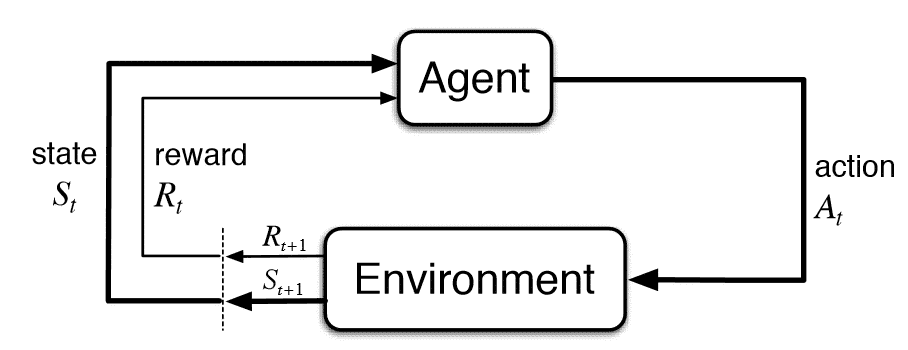
\includegraphics[height=4cm]{img/reinforcement_learning_cycle}
% 	\caption{Reinforcement learning cycle}
% 	\label{fig:reinforcement_learning_cycle}
% \end{figure}
